\documentclass[conference,a4paper]{IEEEtran}
\usepackage[T1]{fontenc}
\usepackage{graphicx}
\usepackage{amsmath}
\usepackage{booktabs}
\usepackage{url}
\renewcommand{\abstractname}{Abstrak}
\renewcommand{\IEEEkeywordsname}{Kata kunci}
\renewcommand{\figurename}{Gambar}
\renewcommand{\tablename}{Tabel}
\renewcommand{\refname}{Referensi}
\title{Analisis Kepadatan dan Klasifikasi Kendaraan pada Lalu Lintas}
\author{\IEEEauthorblockN{\begin{tabular}{@{}c@{\hspace{6mm}}c@{\hspace{6mm}}c@{}}
Hanafi Khairul Shiddiq & Naila Syakira & Helena Koronka Innarmastia
\end{tabular}\\[3pt]
\begin{tabular}{@{}c@{\hspace{6mm}}c@{}}
Gilbard Kinan Nangwaya & Tenno Cahyo Berliantoko
\end{tabular}}
\IEEEauthorblockA{Program Studi Ilmu Komputer, Fakultas Matematika dan Ilmu Pengetahuan Alam\\Universitas Gadjah Mada, Yogyakarta, Indonesia}}
\begin{document}
\raggedbottom
\maketitle

\begin{abstract}
Jumlah kendaraan dan luas jalan yang tampak tertutup dapat memberi gambaran berbeda tentang antrean yang sama. Kami mengembangkan purwarupa untuk menghitung mobil, motor, bus, dan truk serta mengukur cakupan visualnya pada satu foto pendekat persimpangan bersinyal. Pada tiga sudut CCTV di Kabupaten Bantul, detektor klasik memadukan histogram gradien berorientasi, ciri warna, tekstur, dan geometri kamera. Cakupan dihitung dari gabungan kotak kendaraan yang diterima di dalam area jalan. Pada 31 foto uji beranotasi lengkap, galat absolut rata-rata adalah 0,45 kendaraan per foto dan 3,32 poin persentase cakupan. Jumlah total tepat pada 22 foto. Meskipun demikian, pada satu foto dengan hitungan tepat, kotak mobil yang terlalu kecil menyebabkan selisih cakupan 19,17 poin. Pada 76 foto uji dari 55 kelompok adegan, macro-F1 deteksi empat kelas mencapai 59,11\%. F1 mobil dan motor masing-masing melampaui 83\%, sedangkan F1 bus dan truk mencapai 42,86\% dan 23,53\%. Kedua sasaran galat gabungan tercapai pada kamera yang diuji. Kelangkaan contoh kendaraan berat dan kecenderungan meremehkan cakupan di Paseban Barat membatasi penerapannya.
\end{abstract}

\begin{IEEEkeywords}
CCTV lalu lintas, kepadatan visual, klasifikasi kendaraan, histogram gradien berorientasi, mesin vektor pendukung
\end{IEEEkeywords}

\section{Pendahuluan}
Di depan garis henti, beberapa motor dapat berjajar selebar satu mobil. Dari satu foto, jumlah kendaraan menjawab berapa banyak pengguna jalan yang tampak mengantre. Persentase bidang jalan yang tertutup memberi informasi lain. Dua antrean dengan jumlah kendaraan sama bisa tampak sangat berbeda ketika salah satunya berisi sebuah bus. Di sisi lain, dua kotak deteksi yang menandai kendaraan yang sama dapat menambah hitungan tanpa banyak mengubah luas gabungannya. Kedua kemungkinan itu membuat ketepatan hitungan dan ketepatan cakupan perlu dinilai secara terpisah.

CCTV tepi jalan telah digunakan untuk survei kendaraan. Chen \textit{dkk.} memanfaatkan pemodelan latar, klasifikasi jenis kendaraan, dan pelacakan pada urutan gambar~\cite{chen}. Dalam penelitian ini, pengguna hanya memberikan satu foto beserta identitas kamera. Kendaraan yang berhenti tetap perlu ditemukan, termasuk motor yang sebagian tertutup kendaraan lain. Kami menggunakan deskriptor \textit{histograms of oriented gradients} (HOG)~\cite{hog} untuk menggambarkan struktur tepi, serta \textit{support vector machine} (SVM)~\cite{svm} untuk membantu membedakan kandidat kendaraan. Kamera yang tetap memungkinkan model menggunakan letak objek terhadap jalan dan latar referensi yang telah diperoleh dari data latih.

Kajian ini mengajukan tiga pertanyaan. Pertama, seberapa baik model menemukan kendaraan dengan posisi dan kelas yang benar? Kedua, seberapa dekat jumlah per jenis serta persentase cakupan dengan anotasi pada satu pendekat? Ketiga, kesalahan seperti apa yang membuat hitungan tepat sementara luas meleset, atau sebaliknya? Untuk menjawabnya, kami menetapkan batas area ukur pada setiap kamera, menyimpan kotak pembentuk setiap keluaran, dan membandingkan hasil per foto dengan acuan menggunakan aturan geometris yang sama. Persentase yang dihasilkan menyatakan cakupan visual pada saat gambar diambil.

\section{Data dan Metode}
\begin{figure*}[t]
\centering
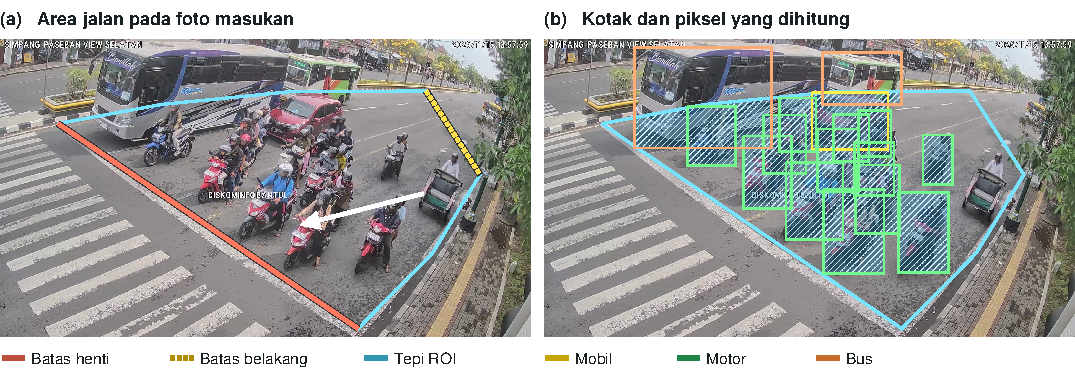
\includegraphics[width=0.98\textwidth]{gambar/S033.pdf}
\caption{Foto validasi S033 dari Paseban Selatan. Pada (a), panah menunjukkan arah menuju batas henti. Pada (b), arsiran mencakup 431.966 dari 727.028 piksel ROI setelah kotak dipotong dan digabungkan. Prediksi terdiri atas 1 mobil, 13 motor, dan 2 bus. Seluruh foto CCTV berasal dari Pemerintah Kabupaten Bantul/Diskominfo Bantul dengan lisensi CC BY 4.0 menurut metadata pemutar saat akuisisi. Penulis menambahkan garis, kotak, dan arsiran.}
\label{fig:roi}
\end{figure*}

\subsection{Pengambilan dan pemilihan foto CCTV}
Kami menggunakan foto dari portal CCTV Pemerintah Kabupaten Bantul~\cite{bantul}. Pemilihan sumber berangkat dari kebutuhan melihat satu pendekat secara utuh, dari batas henti sampai batas belakang pengukuran. Pada percobaan awal dengan citra lalu lintas umum, tersedianya kotak berlabel belum memastikan bahwa batas-batas tersebut terlihat. Pengambilan langsung dari kamera persimpangan memungkinkan kami memeriksa geometri jalan dan membandingkan beberapa tampilan dari antrean yang sama sebelum memilih foto.

Pada 15 November 2026, pengambilan awal menargetkan satu foto setiap lima detik selama sepuluh menit pada lima sudut kamera. Terkumpul 513 gambar. Paseban Selatan menghasilkan 33 gambar karena sumber terputus-putus, sedangkan empat kamera lain masing-masing menghasilkan 120. Banyak gambar berurutan masih menampilkan antrean yang sama. Pengambilan berikutnya menggunakan jendela pengamatan 120 menit, menyimpan segmen sumber dan menghasilkan 1.550 gambar pratinjau dengan interval sasaran sekitar 20 detik. Ketersediaan rekaman berbeda antarkamera. Saat kurasi, perubahan susunan kendaraan dan pergantian antrean membantu membedakan kejadian, dan cuplikan berdekatan dipakai untuk memeriksa objek yang meragukan.

Tiga sudut dipakai pada percobaan foto utuh, yaitu Paseban Selatan dan Paseban Barat di satu simpang, serta Bejen Barat di simpang lain. Pada sudut Klodran, sebagian batas area henti terpotong sehingga sudut itu disimpan sebagai cadangan. Foto Palbapang menyumbang contoh tambahan untuk pelatihan klasifikasi. Pada foto yang dipilih, kabel, marka aus, bayangan, serta kendaraan yang berhimpitan tetap terlihat sebagaimana terekam oleh CCTV. Kondisi ini penting karena tepi yang kuat pada citra juga dapat berasal dari benda di luar kendaraan.

Kurasi awal memilih 26 foto untuk menguji aturan anotasi. Dari pengamatan 120 menit, 38 foto dipilih sebagai himpunan awal. Cakupannya kemudian diperluas menjadi 222 foto dari tiga sudut utama, termasuk keadaan kosong dan adegan dengan kendaraan bertumpuk. Paket eksperimen akhir memuat 248 foto inti setelah penambahan 26 foto. Dua belas contoh tambahan dari Palbapang dikhususkan untuk klasifikasi di sisi latih. Jumlah foto pada tahapan tersebut merujuk pada himpunan yang saling beririsan.

\subsection{Area pengukuran dan anotasi kendaraan}
Gambar~\ref{fig:roi}(a) memperlihatkan batas area ukur di Paseban Selatan. Setiap kamera memiliki poligon tetap pada permukaan jalan, yang selanjutnya disebut ROI (\textit{region of interest}). Batas depannya mengikuti garis henti atau batas henti yang ditetapkan pada referensi kamera. Batas belakang virtual membatasi panjang pendekat yang bisa dibandingkan antarfoto. Trotoar, median, dan jalan arah sebaliknya berada di luar poligon. Pada resolusi asli, luas ROI Paseban Selatan dan Paseban Barat masing-masing 727.028 dan 134.972 piksel pada citra $1920\times1080$. ROI Bejen Barat mencakup 114.721 piksel pada citra $1280\times720$. Penyebut luas yang berbeda ini mengikuti geometri pendekat pada masing-masing sudut.

Anotasi memuat kotak pembatas, kelas, dan keputusan apakah objek berada pada pendekat. Dalam 26 gambar percobaan, penggunaan pusat kotak sebagai penentu keanggotaan menghasilkan 34 pengecualian keliru dan satu penerimaan keliru dibandingkan dengan pemeriksaan posisi fisik. Atap kendaraan yang tinggi, misalnya, dapat terproyeksi ke median pada gambar meskipun rodanya masih berada di jalur sasaran. Karena itu, peninjauan memperhatikan posisi roda, alas kendaraan, serta bukti visual di sekitar batas. Jika objek tertutup dan kedudukannya tidak dapat dipastikan, area tersebut ditandai ambigu.



Dalam paket 222 foto, 87 foto mempunyai acuan hitungan lengkap dan 135 foto memiliki label parsial. Paket tersebut memuat 2.087 kotak, termasuk objek konteks. Kelas sasaran adalah mobil, motor, bus, dan truk. Kotak motor mencakup bagian pengendara dan penumpang yang terlihat. Pikap atau van kargo yang ditetapkan sebagai kelas lain tetap dicatat sebagai objek pembanding. Anotasi serta peninjauan silang menggunakan bantuan AI. Penilaian antarpemberi label manusia secara independen belum tersedia. Perbedaan status lengkap dan parsial menentukan ukuran yang bisa dinilai pada tiap foto.

\subsection{Mendeteksi dan mengklasifikasikan kendaraan}
Detektor memeriksa kandidat kotak pada delapan tinggi jendela dan lima rasio aspek di sekitar ROI. Setiap kandidat dinormalkan ke jendela $64\times64$ piksel untuk menghitung HOG, menggunakan sel $8\times8$, blok $16\times16$, serta sembilan arah gradien. HOG menangkap susunan tepi seperti kontur badan kendaraan. Warna, pola biner lokal untuk tekstur, selisih terhadap latar median kamera, ukuran kandidat, dan posisi dalam gambar melengkapi deskripsi tersebut. Latar referensi dibentuk dari foto latih sehingga saat inferensi pengguna cukup memasukkan satu foto baru.

SVM memberi skor kelas. Penilai lokasi berbasis pohon keputusan (\textit{boosting} dan ExtraTrees) memperkirakan seberapa rapat setiap kandidat membingkai kendaraan. Selama pelatihan, potongan kendaraan utuh menjadi contoh positif. Contoh negatif mencakup latar yang diketahui serta fragmen kendaraan yang dapat mengecoh detektor, seperti sebagian sisi bus yang menyerupai badan truk. Setelah penilaian, regresi mengoreksi koordinat kotak. Dukungan kandidat yang saling berimpit membantu menentukan posisi akhir dan menekan deteksi berulang. Pemilihan ambang dilakukan pada data validasi.

Baseline HOG dan SVM awal setelah kalibrasi mencapai macro-F1 validasi 7,33\%. Dalam diagnosis baseline itu, grid kandidat telah menjangkau 573 dari 574 objek validasi dengan tumpang tindih minimal 0,50. Temuan ini mengarahkan percobaan berikutnya pada pemilihan kandidat dan koreksi posisi kotak. Konfigurasi v35 mencapai 84,91\% di validasi setelah beberapa perubahan pada fitur, penilaian lokasi, pelatihan kendaraan berat, dan penggabungan kandidat. Konfigurasi akhir v45 menambahkan koreksi halus kotak motor berbasis regresi Ridge dan pemeriksa fragmen berbasis SVM, lalu mencapai 85,50\%. Perbandingan antartonggak ini menggambarkan pemilihan sistem secara keseluruhan. Beberapa komponen berubah bersama sehingga pengaruh setiap komponen belum terisolasi.

\subsection{Menghitung jumlah dan kepadatan visual}
Untuk foto baru, model menentukan keanggotaan ROI dari perkiraan titik kontak dengan jalan. Pada kedua kamera Paseban digunakan koreksi posisi titik kontak yang dipelajari dari data latih. Bejen menggunakan aturan yang mengacu pada bagian bawah kotak. Satu daftar deteksi yang diterima kemudian menjadi dasar kedua keluaran. Dengan $A$ sebagai himpunan deteksi yang diterima, $c_i$ kelas deteksi ke-$i$, $B_i$ piksel di dalam kotaknya, dan $R$ masker jalan, hitungan per kelas dan cakupan visual adalah
\begin{align}
N_c &= \sum_{i\in A}\mathbf{1}(c_i=c), \label{eq:count}\\
D &= 100\,\frac{\left|R\cap\bigcup_{i\in A}B_i\right|}{|R|},\qquad |R|>0. \label{eq:area}
\end{align}
Persamaan~(\ref{eq:area}) memberi bobot satu pada setiap piksel yang tertutup, berapa pun jumlah kotak yang menutupinya. Jika $R$ valid dan $A$ kosong, $N_c$ dan $D$ sama dengan nol. Persentase tidak terdefinisi untuk masker jalan berluas nol. Kotak berbentuk persegi panjang juga dapat mencakup ruang di samping roda atau di atas bodi. Perspektif membuat kendaraan dekat kamera menempati lebih banyak piksel. Dengan demikian, pengukuran ini memiliki satuan persen dari bidang citra jalan. Kepadatan dalam kendaraan per kilometer memerlukan kalibrasi jarak dan definisi pengukuran tersendiri.

Pada contoh validasi di Gambar~\ref{fig:roi}, anotasi dan model sama-sama memberi total 16 kendaraan. Gabungan kotak acuan menutup 441.898 piksel (60,78\%), sedangkan kotak prediksi menutup 431.966 piksel (59,42\%). Selisih bersih 9.932 piksel muncul walaupun hitungan setiap kelas tepat. Masker yang disimpan bersama prediksi memungkinkan pembaca menelusuri selisih itu sampai ke gambar asal.

\section{Rancangan Evaluasi}
\subsection{Pembagian data dan pembekuan model}
Foto yang berpotensi memuat antrean atau kendaraan yang sama diikat dalam satu kelompok sebelum data dibagi. Pengelompokan mempertimbangkan waktu rekaman, pergantian kendaraan, dan hubungan antarsudut. Dua kamera di Paseban, misalnya, tidak otomatis menghasilkan dua kejadian independen. Paket inti memberi 99 foto untuk latih, 61 untuk validasi, dan 76 untuk uji. Sepuluh foto berada dalam jeda pemisah waktu dan dua foto dikarantina karena identitas kendaraan meragukan. Semua sudut dalam uji telah dikenal model saat pelatihan.

Fitur, contoh pelatihan, dan latar referensi bersumber dari sisi latih. Validasi digunakan berulang untuk memilih ambang dan konfigurasi. Potongan tambahan serta variasi kecil posisi kotak dapat menambah contoh fitur selama pelatihan, tetapi beberapa variasi dari satu kendaraan tetap mewakili satu pengamatan sumber. Konfigurasi v45 beserta pembanding v35 dikunci sebelum evaluasi uji. Seluruh prediksi uji disimpan terlebih dahulu, kemudian dicocokkan dengan acuan. Uji mencakup 55 kelompok adegan. Dari 76 foto, 66 berasal dari 15 November dan 10 dari 17 November 2026.

\subsection{Pencocokan objek dan pengukuran galat}
Untuk deteksi, urutan skor menentukan pencocokan satu lawan satu. Suatu prediksi menjadi deteksi benar jika kelasnya sama dengan acuan dan rasio luas irisan terhadap gabungan kedua kotak (\textit{intersection over union}, IoU) mencapai 0,50. Evaluasi berbasis kelas dan tumpang tindih mengikuti prinsip evaluasi deteksi objek~\cite{voc}. Prediksi kedua atas acuan yang telah berpasangan dihitung berlebih. Pada 45 foto parsial, prediksi yang memenuhi aturan zona ambigu boleh berstatus netral. Objek yang diketahui termasuk kelas lain tetap dapat menghasilkan alarm palsu. Dengan aturan ini, keempat kelas dapat dievaluasi pada 76 foto meskipun sebagian area pada sejumlah foto belum dapat diberi acuan lengkap.

Presisi menyatakan proporsi prediksi yang benar, sedangkan \textit{recall} menyatakan proporsi objek acuan yang ditemukan. F1 adalah rata-rata harmonik keduanya. Macro-F1 menghitung rata-rata F1 keempat kelas dengan bobot sama. Interval deskriptif 95\% diperoleh dengan 2.000 pengambilan ulang atas kelompok adegan, dengan kelompok lintas kamera tetap utuh. Untuk menelaah salah kelas, kami juga melakukan pencocokan terpisah berdasarkan urutan IoU tertinggi tanpa syarat kelas. Tabel diagnosis ini menunjukkan tujuan pasangan setiap objek acuan dan menggunakan prosedur terpisah dari perhitungan F1 resmi.

Untuk hitungan dan cakupan, evaluasi dibatasi pada 31 foto dengan acuan lengkap. Galat absolut rata-rata (MAE) dihitung untuk jumlah total, hitungan tiap kelas, dan persentase cakupan. Jika $y_j$ adalah acuan dan $\hat y_j$ prediksi pada foto $j$, maka
\begin{equation}
\mathrm{MAE}=\frac{1}{n}\sum_{j=1}^{n}|\hat y_j-y_j|. \label{eq:mae}
\end{equation}
Setiap foto mendapat bobot sama dalam hasil gabungan. Kami juga menghitung rata-rata selisih bertanda untuk melihat kecenderungan nilai cakupan terlalu tinggi atau terlalu rendah. Sasaran yang ditetapkan sebelum uji adalah MAE total paling banyak satu kendaraan per foto, MAE cakupan paling banyak lima poin persentase, macro-F1 minimal 85\%, dan F1 minimal 75\% untuk setiap kelas.

\section{Hasil dan Pembahasan}
\subsection{Ketepatan jumlah kendaraan dan cakupan jalan}
Dua sasaran galat gabungan tercapai (Tabel~\ref{tab:area}). Model memberi jumlah total tepat pada 22 dari 31 foto dan jumlah tepat untuk keempat kelas sekaligus pada 21 foto. Galat absolut rata-rata per foto adalah 0,13 mobil, 0,32 motor, 0,06 bus, dan 0,06 truk. Angka yang kecil untuk kendaraan berat perlu dibaca bersama frekuensi kemunculannya. Dalam himpunan acuan lengkap, hanya dua foto yang memuat bus dan dua foto yang memuat truk. Foto tanpa objek dari suatu kelas juga berkontribusi pada penghitungan MAE kelas tersebut.

\begin{table}[tb]
\centering
\caption{Hitungan dan cakupan pada 31 foto uji dengan acuan lengkap}
\label{tab:area}
\footnotesize\setlength{\tabcolsep}{4pt}
\begin{tabular}{lrrrr}\toprule
Kamera & Foto & Total tepat & MAE $N$ & MAE $D$\\
 & & (foto) & (kend./foto) & (poin pers.)\\\midrule
Paseban Selatan & 12 & 8 & 0,67 & 1,86\\
Paseban Barat & 11 & 8 & 0,27 & 6,63\\
Bejen Barat & 8 & 6 & 0,38 & 0,93\\\midrule
Gabungan & 31 & 22 & 0,45 & 3,32\\\bottomrule
\end{tabular}
\end{table}

Pada lima foto yang memang kosong, keluaran model juga nol. Jika hanya 26 foto berisi kendaraan yang dihitung, MAE menjadi 0,54 kendaraan dan 3,95 poin persentase. Cakupan model berada di bawah acuan pada 23 foto, di atas acuan pada tiga foto, dan sama pada lima foto kosong. Bias rata-rata adalah $-3{,}21$ poin persentase. Perbedaan antarkamera paling jelas terlihat di Paseban Barat. Di sana jumlah total tepat pada delapan dari sebelas foto, sedangkan cakupan terlalu rendah pada kesepuluh foto yang memuat kendaraan. Rata-rata galat cakupan di sudut tersebut mencapai 6,63 poin persentase, lebih besar daripada di kedua sudut lainnya.

\begin{figure}[tb]
\centering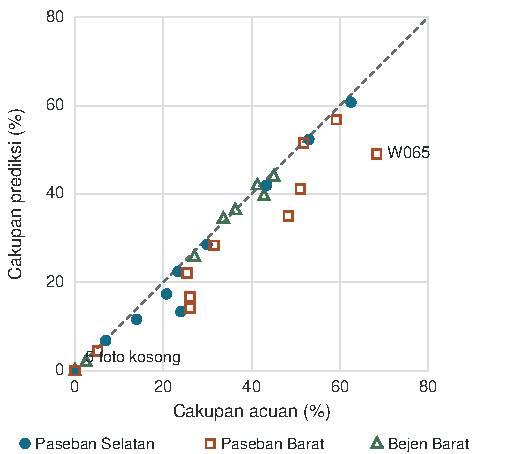
\includegraphics[width=0.95\columnwidth]{gambar/Cakupan31.pdf}
\caption{Cakupan prediksi terhadap acuan pada 31 foto. Garis putus-putus menandai kesetaraan. Titik di bawah garis berarti cakupan terlalu rendah. Lima foto kosong berimpit pada titik asal. W065 adalah foto dengan galat cakupan terbesar.}
\label{fig:scatter}
\end{figure}

Sebaran pada Gambar~\ref{fig:scatter} menunjukkan mengapa satu nilai MAE belum cukup menggambarkan perilaku sistem. Dua kamera dapat memiliki kesalahan jumlah yang serupa dengan kesalahan luas berbeda. Di samping pengaruh perspektif, ukuran satu kotak mobil di bagian depan antrean dapat memengaruhi banyak piksel sekaligus. Besarnya kontribusi masing-masing faktor pada perbedaan antarkamera belum diisolasi melalui percobaan tersendiri.

\begin{figure*}[t]
\centering
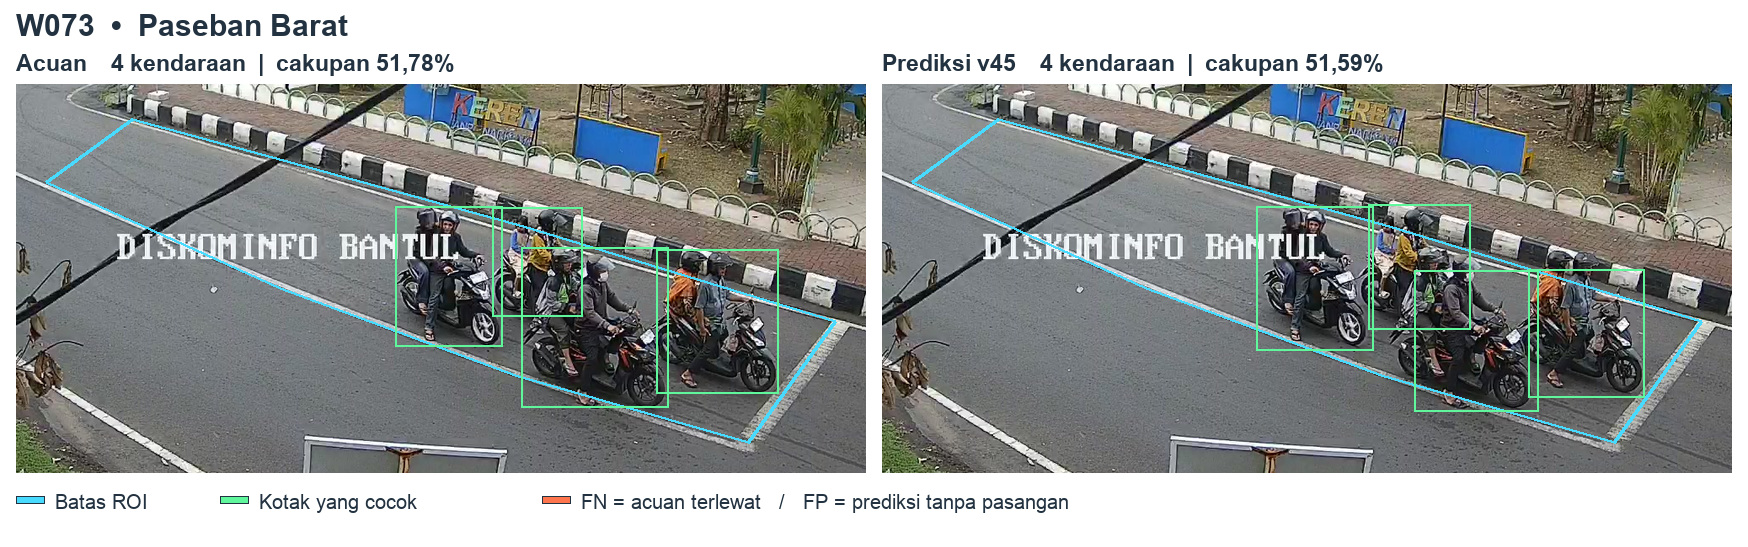
\includegraphics[width=.89\textwidth]{gambar/W073.jpg}\par\smallskip
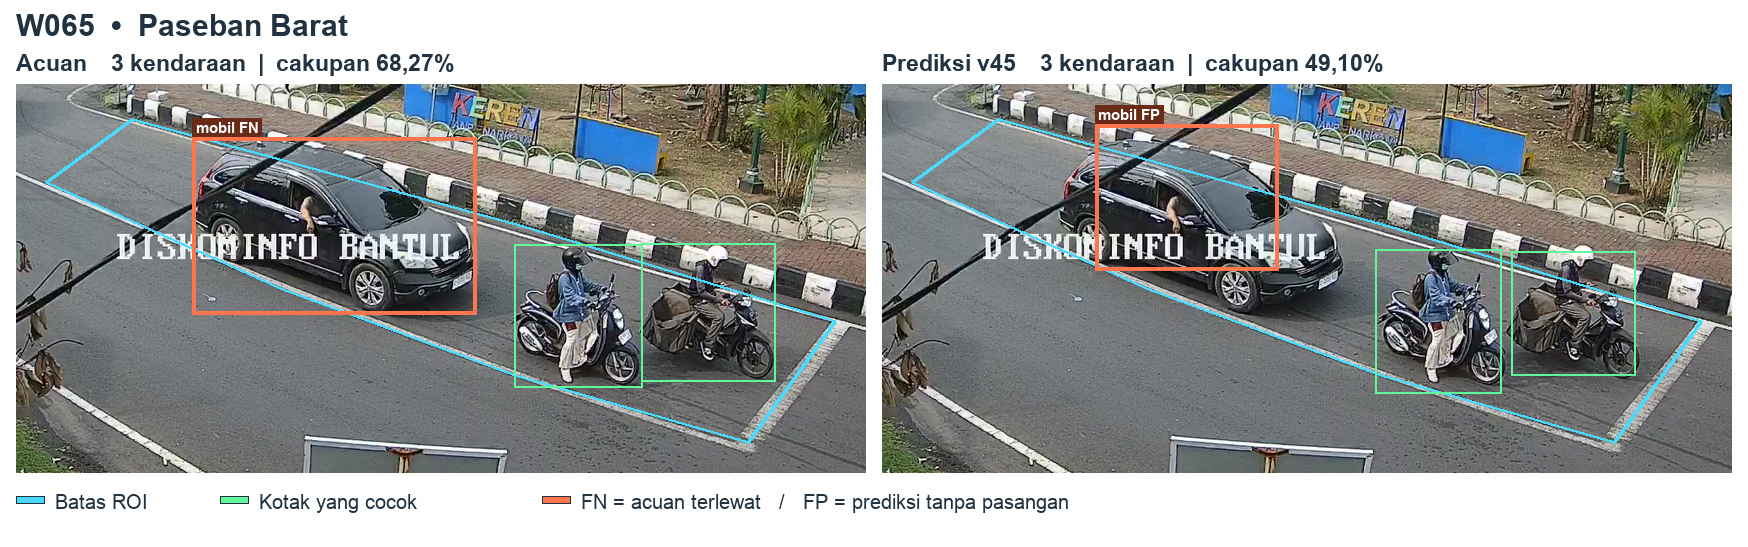
\includegraphics[width=.89\textwidth]{gambar/W065.jpg}
\caption{Acuan (kiri) dan prediksi (kanan) pada dua foto uji Paseban Barat. Pada W073 (atas), empat motor cocok. Pada W065 (bawah), ujung kotak prediksi mobil berada di tengah badan kendaraan. Garis biru menandai ROI. Kotak hijau memiliki pasangan benar, sedangkan jingga menandai acuan yang terlewat atau prediksi berlebih. Foto CCTV dipotong pada bidang pandang yang sama dalam setiap pasangan dan diberi anotasi oleh penulis. Kredit dan lisensi mengikuti Gambar~\ref{fig:roi}.}
\label{fig:cases}
\end{figure*}

\subsection{Ketepatan deteksi empat kelas}
Pada data validasi, macro-F1 sebesar 85,50\%. Pada uji terpisah, macro-F1 sebesar 59,11\% dengan interval bootstrap kelompok 45,81--66,30\%. Hasil validasi mencerminkan konfigurasi yang dipilih setelah beberapa putaran pengembangan. Hasil uji menjadi dasar penilaian akhir. Konfigurasi pembanding v35 memberi macro-F1 uji 58,28\%. Dibandingkan dengan v35, v45 meningkatkan macro-F1 uji sekitar 0,83 poin persentase. F1 kedua kelas berat tetap sama pada kedua konfigurasi.

\begin{table}[tb]
\centering\caption{Deteksi per kelas pada 76 foto uji dengan IoU minimal 0,50}
\label{tab:det}
\footnotesize\setlength{\tabcolsep}{4.2pt}
\begin{tabular}{lrrrrr}\toprule
Kelas & Acuan & Benar & Presisi (\%) & Recall (\%) & F1 (\%)\\\midrule
Mobil & 148 & 130 & 84,42 & 87,84 & 86,09\\
Motor & 439 & 361 & 85,75 & 82,23 & 83,95\\
Bus & 8 & 3 & 50,00 & 37,50 & 42,86\\
Truk & 6 & 2 & 18,18 & 33,33 & 23,53\\\bottomrule
\end{tabular}
\end{table}

Mobil dan motor menyumbang 587 dari 601 objek acuan (Tabel~\ref{tab:det}). Ketika seluruh objek digabungkan, micro-F1 mencapai 83,15\%. Macro-F1 memberi bobot yang sama pada bus dan truk sehingga memperlihatkan kesulitan yang kurang tampak pada nilai gabungan per objek. Dari enam truk acuan, dua terdeteksi dengan kelas dan posisi yang benar. Sembilan kotak tambahan diberi kelas truk secara keliru. Karena dukungan bus dan truk kecil, tambahan satu pasangan benar saja dapat mengubah recall kelas secara besar. Hasil uji belum mencapai sasaran macro-F1 maupun sasaran F1 untuk keempat kelas sekaligus.

\begin{table}[tb]
\centering\caption{Pasangan lokasi tanpa syarat kelas pada 76 foto uji}
\label{tab:diag}
\footnotesize\setlength{\tabcolsep}{4pt}
\begin{tabular}{lrrrrr}\toprule
 & \multicolumn{4}{c}{Kelas prediksi pada kotak pasangan} & Tanpa\\
Acuan & Mobil & Motor & Bus & Truk & pasangan\\\midrule
Mobil & 130 & 0 & 0 & 0 & 18\\
Motor & 0 & 361 & 0 & 0 & 78\\
Bus & 0 & 0 & 3 & 1 & 4\\
Truk & 1 & 0 & 0 & 2 & 3\\\bottomrule
\end{tabular}
\end{table}

Pencocokan tanpa syarat kelas membantu membedakan dua bentuk kegagalan (Tabel~\ref{tab:diag}). Satu bus memiliki pasangan yang dinilai sebagai truk, sedangkan satu truk memiliki pasangan yang dinilai sebagai mobil. Empat bus dan tiga truk lainnya tidak memperoleh pasangan pada IoU minimal 0,50. Ketiadaan pasangan dapat terjadi jika objek terlewat atau kotaknya kurang tepat. Matriks ini hanya memiliki baris untuk objek acuan sehingga prediksi berlebih tanpa pasangan tidak tercantum. Presisi dan F1 pada Tabel~\ref{tab:det} memperhitungkan prediksi berlebih sesuai protokol resmi.

Percobaan lanjutan memperlihatkan kesulitan membedakan truk dari pikap boks dan potongan badan bus. Pada sebelas foto siang di luar uji resmi, penambahan pembeda truk dan koreksi tepi kotak tetap menemukan satu dari dua truk, sementara alarm palsu truk naik dari satu menjadi delapan. Hasil ini menjelaskan mengapa kami mempertahankan v45 untuk demo dan evaluasi akhir.

\subsection{Mengapa hitungan dan luas dapat berbeda}
Gambar~\ref{fig:cases} membandingkan dua foto Paseban Barat dengan aturan ROI yang sama. Pada W073, keempat motor terdeteksi pada kelas dan posisi yang sesuai. Cakupan prediksi 51,59\% mendekati acuan 51,78\%. Selisih bersihnya 255 piksel. Pada W065, acuan dan prediksi sama-sama memberi satu mobil dan dua motor. Kotak mobil hanya menutup sebagian badan kendaraan dan IoU-nya 0,463. Pada evaluasi deteksi, mobil acuan tercatat terlewat dan prediksi mobil tercatat berlebih. Pada evaluasi jumlah, keduanya saling mengimbangi. Pada evaluasi cakupan, kotak yang terlalu kecil menurunkan hasil dari 68,27\% menjadi 49,10\%, selisih 19,17 poin persentase.



Kebalikan pola W065 tampak pada S059 di Paseban Selatan. Model menghitung 23 kendaraan terhadap 19 pada acuan. Lima kotak berlebih dan satu mobil yang terlewat menaikkan jumlah bersih empat kendaraan. Namun, dari 121.518 piksel di dalam ROI yang ditutup gabungan kotak berlebih, hanya 3.844 berada di luar kotak prediksi yang sudah berpasangan benar. Akibatnya, cakupan prediksi 60,81\% tetap dekat dengan acuan 62,48\%. Dengan demikian, hitungan terlalu tinggi sementara luas terlalu rendah. Pada empat dari 22 foto dengan total tepat, deteksi berlebih dan objek terlewat juga muncul bersamaan.

Kasus-kasus tersebut dipilih setelah evaluasi untuk menelaah cara kesalahan terbentuk. W065 dan S059 memberikan galat absolut terbesar masing-masing untuk cakupan dan total hitungan. W073 memberikan galat cakupan terkecil di antara foto berisi kendaraan yang semua deteksinya berpasangan benar. Tabel per kamera dan sebaran seluruh 31 foto memperlihatkan seberapa jauh satu kasus berbeda dari sampel selebihnya.

\subsection{Waktu proses, keterulangan, dan batas penerapan}
Pada 76 foto uji, median inferensi adalah 8,10 detik per foto dan persentil ke-90 sebesar 20,94 detik pada macOS arm64 dengan satu \textit{thread} komputasi untuk OpenCV dan pustaka numerik. Waktu dihitung setelah foto RGB dan model tersedia. Interval mencakup deteksi, penyalinan hasil pembanding pada uji berpasangan, koreksi kotak, dan perhitungan keluaran. Pembacaan dan penyimpanan berkas serta penggambaran hasil berada di luar pengukuran.

Kesesuaian kamera memengaruhi hasil lebih awal daripada klasifikasi. Dalam audit penggunaan, piksel foto Paseban Barat W046 disimpan sebagai PNG dan diberikan ke demo dengan dua pilihan kamera. Pilihan yang benar memberi tiga motor dan cakupan 33,09\%. Ketika pilihan diubah ke Paseban Selatan, berkas yang sama diterima dan menghasilkan 31 motor, dua truk, dan cakupan 50,66\%. Kedua kamera memiliki resolusi sama, tetapi area ukur dan latar referensinya berbeda. Untuk foto baru, pengguna perlu mencocokkan sudut pengambilan dan posisi batas jalan dengan referensi kamera.

Komposisi data juga membatasi interpretasi. Pada himpunan uji lengkap, 22 dari 31 foto memuat paling banyak empat kendaraan, dan hanya dua yang memuat lebih dari sepuluh. Jalan yang padat dengan kendaraan saling menutupi lebih sulit diberi acuan lengkap. Dengan demikian, hasil untuk 31 foto ini belum membuktikan bahwa galat rata-rata yang sama akan diperoleh pada antrean yang lebih padat. Pemisahan berdasarkan kelompok memberi pengujian pada kejadian yang terpisah di kamera yang sudah dikenal. Kinerja pada sudut baru serta kesepakatan antarpenilai manusia merupakan dua pertanyaan yang masih terbuka.

Kode inferensi, kartu data, dan tabel evaluasi tersedia pada repositori tim~\cite{repo}. Paket demo Mac Apple Silicon menyediakan model dan empat foto validasi. Pengujian dari direktori bersih dengan akses jaringan dan akses ke folder proyek asal diblokir menghasilkan kotak, kelas, hitungan, dan piksel masker yang cocok dengan keluaran beku untuk keempat contoh. Bukti tersebut mencakup inferensi. Pelatihan ulang seluruh rangkaian model dari ruang kerja kosong masih memerlukan artefak pengembangan tambahan.

\section{Kesimpulan}
Pada tiga sudut CCTV Bantul yang dikenal model, pendekatan pengolahan citra klasik menghasilkan hitungan dan cakupan jalan dengan MAE gabungan 0,45 kendaraan per foto dan 3,32 poin persentase pada 31 foto uji beracuan lengkap. Untuk deteksi empat kelas pada 76 foto uji, macro-F1 mencapai 59,11\%. Mobil dan motor lebih sering ditemukan dengan kelas dan lokasi yang benar daripada bus dan truk.

\newpage
Hubungan antara kotak dan keluaran menjelaskan mengapa dua sasaran galat gabungan dapat tercapai walaupun kemampuan deteksi empat kelas masih terbatas. Kotak mobil yang terlalu pendek dapat mengurangi luas secara nyata tanpa mengubah jumlah. Di sisi lain, kotak tambahan yang bertumpuk dapat menaikkan hitungan dengan sedikit perubahan luas. Untuk menilai kesiapan penggunaan di luar tiga sudut ini, pengujian selanjutnya perlu mencakup sesi dan sudut lain, antrean padat dengan beragam bus dan truk, serta anotasi yang diperiksa penilai manusia independen.

\begin{thebibliography}{00}
\bibitem{chen} Z. Chen, T. Ellis, and S. A. Velastin, ``Vision-based traffic surveys in urban environments,'' \textit{J. Electron. Imaging}, vol. 25, no. 5, Art. no. 051206, 2016, doi: 10.1117/1.JEI.25.5.051206.
\bibitem{hog} N. Dalal and B. Triggs, ``Histograms of oriented gradients for human detection,'' in \textit{Proc. IEEE Comput. Soc. Conf. Comput. Vis. Pattern Recognit.}, vol. 1, 2005, pp. 886--893, doi: 10.1109/CVPR.2005.177.
\bibitem{svm} C. Cortes and V. Vapnik, ``Support-vector networks,'' \textit{Mach. Learn.}, vol. 20, no. 3, pp. 273--297, 1995, doi: 10.1007/BF00994018.
\bibitem{bantul} Pemerintah Kabupaten Bantul, ``CCTV Bantul.'' [Daring]. Tersedia pada \url{https://bantulkab.go.id/cctv.html}. Diakses 19 November 2026. Lisensi pada pemutar: \url{https://creativecommons.org/licenses/by/4.0/}.
\bibitem{voc} M. Everingham, L. Van Gool, C. K. I. Williams, J. Winn, and A. Zisserman, ``The PASCAL Visual Object Classes (VOC) Challenge,'' \textit{Int. J. Comput. Vis.}, vol. 88, no. 2, pp. 303--338, 2010, doi: 10.1007/s11263-009-0275-4.
\bibitem{repo} H. K. Shiddiq, N. Syakira, H. K. Innarmastia, G. K. Nangwaya, dan T. C. Berliantoko, ``Analisis kepadatan dan klasifikasi kendaraan pada lalu lintas,'' kode inferensi, kartu dataset, dan hasil evaluasi, rilis v45, 2026. [Daring]. \url{https://github.com/hanafishiddiq/tugas-akhir-pcd}.
\end{thebibliography}
\end{document}
